\documentclass[14pt, a4paper]{report}
\usepackage{mathtext}
\usepackage[T2A]{fontenc}
\usepackage[utf8]{inputenc}
\usepackage[russian]{babel}
\usepackage{multirow}
\usepackage{slashbox}
\usepackage{makecell}
\usepackage{graphicx}
\usepackage{physics}
\usepackage{amstext}
\usepackage{caption}
\usepackage{subcaption}
\usepackage{cmap}
\usepackage{float}
\usepackage{indentfirst}

\usepackage[a4paper,
            		left=1in,
            		right=1in,
           		 top=1in,
            		bottom=1in,
            		footskip=.25in]{geometry}

\renewcommand{\thesection}{\arabic{section}.}
\renewcommand{\thesubsection}{\arabic{section}.\arabic{subsection}.}
\pagenumbering{arabic}

\title{\textbf{Отчет о выполнении лабораторной работы 2.1 "Опыт Франка-Герца"}}
\author{Калашников Михаил, Б03-202}
\date{}

\begin{document}
\maketitle

\textbf{Цель работы:}
Измерение энергиии первого уровня атома гелия методом электронного возбуждения в динамическом и статическом режимах.
\newline

\section{Теоретические сведения}

Опыт Франка и Герца является одним из самых простых опытов, подтверждающих существование дискретных уровней энергии атомов.

Разреженный гелий заполняет трехэлектродную лампу. Электроны ускоряются в постоянном электрическом поле, созданным между катодом и анодом лампы. Передвигаясь от катода к аноду, электроны сталкиваются с атомами гелия. При энергии, недостаточной для ионизации атома гелия, происходят упругии соударения, при которых электроны практически не теряют энергии.

\begin{figure}[H]
\centering
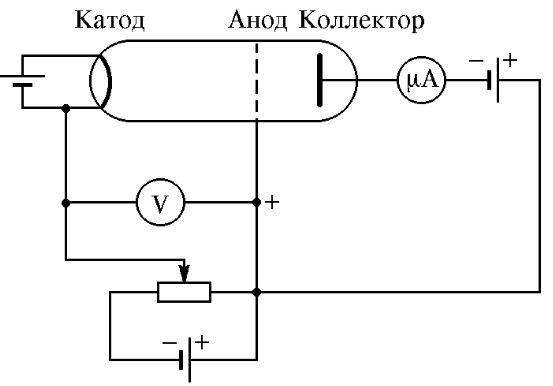
\includegraphics[scale=0.6]{../images/521-1}
\caption{Принципиальная схема опыта Франка и Герца}
\end{figure}

По мере увеличения разности потенциалов между анодом и катодом энергия электронов становится достаточной для возбуждения атомов. При таких неупругих столкновениях кинетическая энергия налетающего электрона передается одному из атомных электронов, вызывая его переход на свободный энергетический уровень или совсем отрывая его от атома.

При увеличении потенциала анода ток коллектора вначале растет. Однако, когда энергия электронов становится достаточной для возбужения атомов, ток коллектора резко уменьшается из-за того, что претерпевшие неупругое соударение электроны не могут преодолеть задерживающее напряжение.

\begin{figure}[H]
\centering
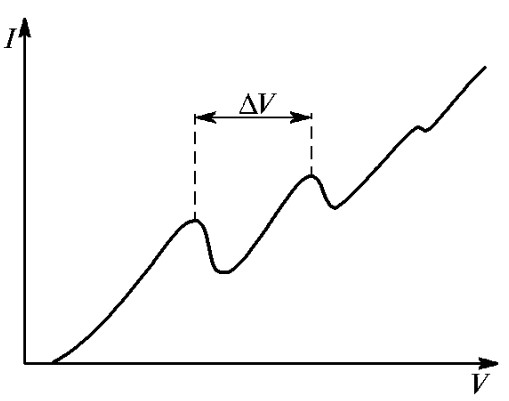
\includegraphics[scale=0.6]{../images/521-2}
\caption{Зависимость тока коллектора от напряжения на аноде}
\end{figure}

\section{Экспериментальная установка}

Для опыта используется серийная лампа ионизационного манометра ЛМ-2, заполненная гелием до давления ~1 Торр. Источником электронов является вольфрамолый катод, нагреваемый переменным током. Ток накала регулируется амперметром А. Ускоряющее напряжение подается на анод от выпрямителя В. Источник задерживающего напряжения -- батарея 4.5 В.

\begin{figure}[H]
\centering
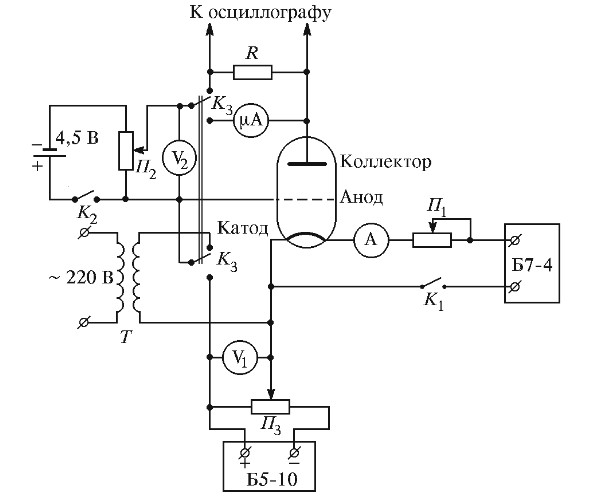
\includegraphics[scale=0.6]{../images/521-3}
\caption{Схема экспериментальной установки}
\end{figure}

Схему можно переключать из статического режима измерений в динамический  с помощью ключа $К_3$. При динамическом режиме ускоряющий потенциал подается с понижающего трансформатора Т.

\section{Проведение эксперимента}

\begin{enumerate}

\item Подготовим приборы к работе. Включим и настроим электронный осциллограф.

\item Настроим установку на динамический режим работы. Пронаблюдаем полную картину АЧХ при трех различных значения задерживающего напряжения.

\begin{figure}[H]
\centering
\begin{subfigure}{.33\textwidth}
  \centering
  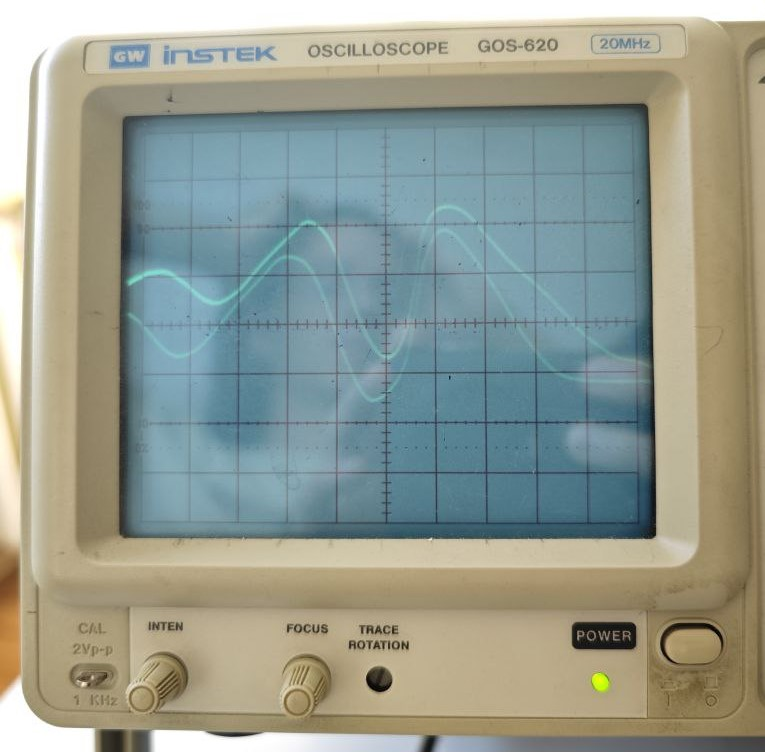
\includegraphics[width=.975\linewidth]{../images/521-8a}
\end{subfigure}%
\begin{subfigure}{.33\textwidth}
  \centering
  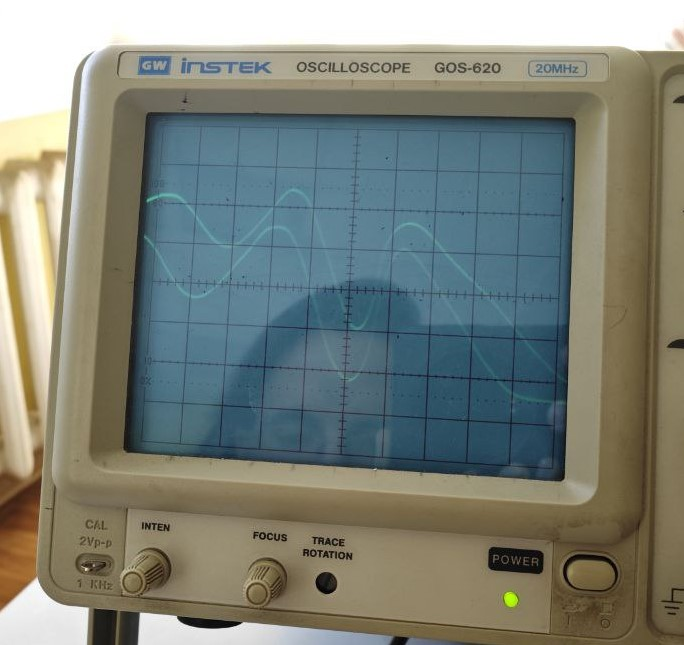
\includegraphics[width=.975\linewidth]{../images/521-8b}
\end{subfigure}%
\begin{subfigure}{.33\textwidth}
  \centering
  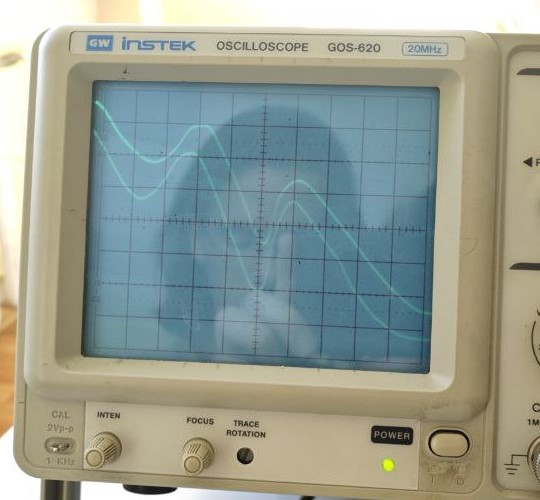
\includegraphics[width=.975\linewidth]{../images/521-8c}
\end{subfigure}
\caption{АЧХ в динамическом режиме при $U_{зад}=4,\ 6,\ 8\ В$}
\end{figure}

\item Переведем установку в статический режим.

\item Для каждого значения задерживающего напряжения снимем зависимость коллекторного тока от анодного напряжения. Особенно тщательно проведем измерения в тех областях где наблюдаются максимумы и минимумы тока.

\begin{figure}[H]
\centering
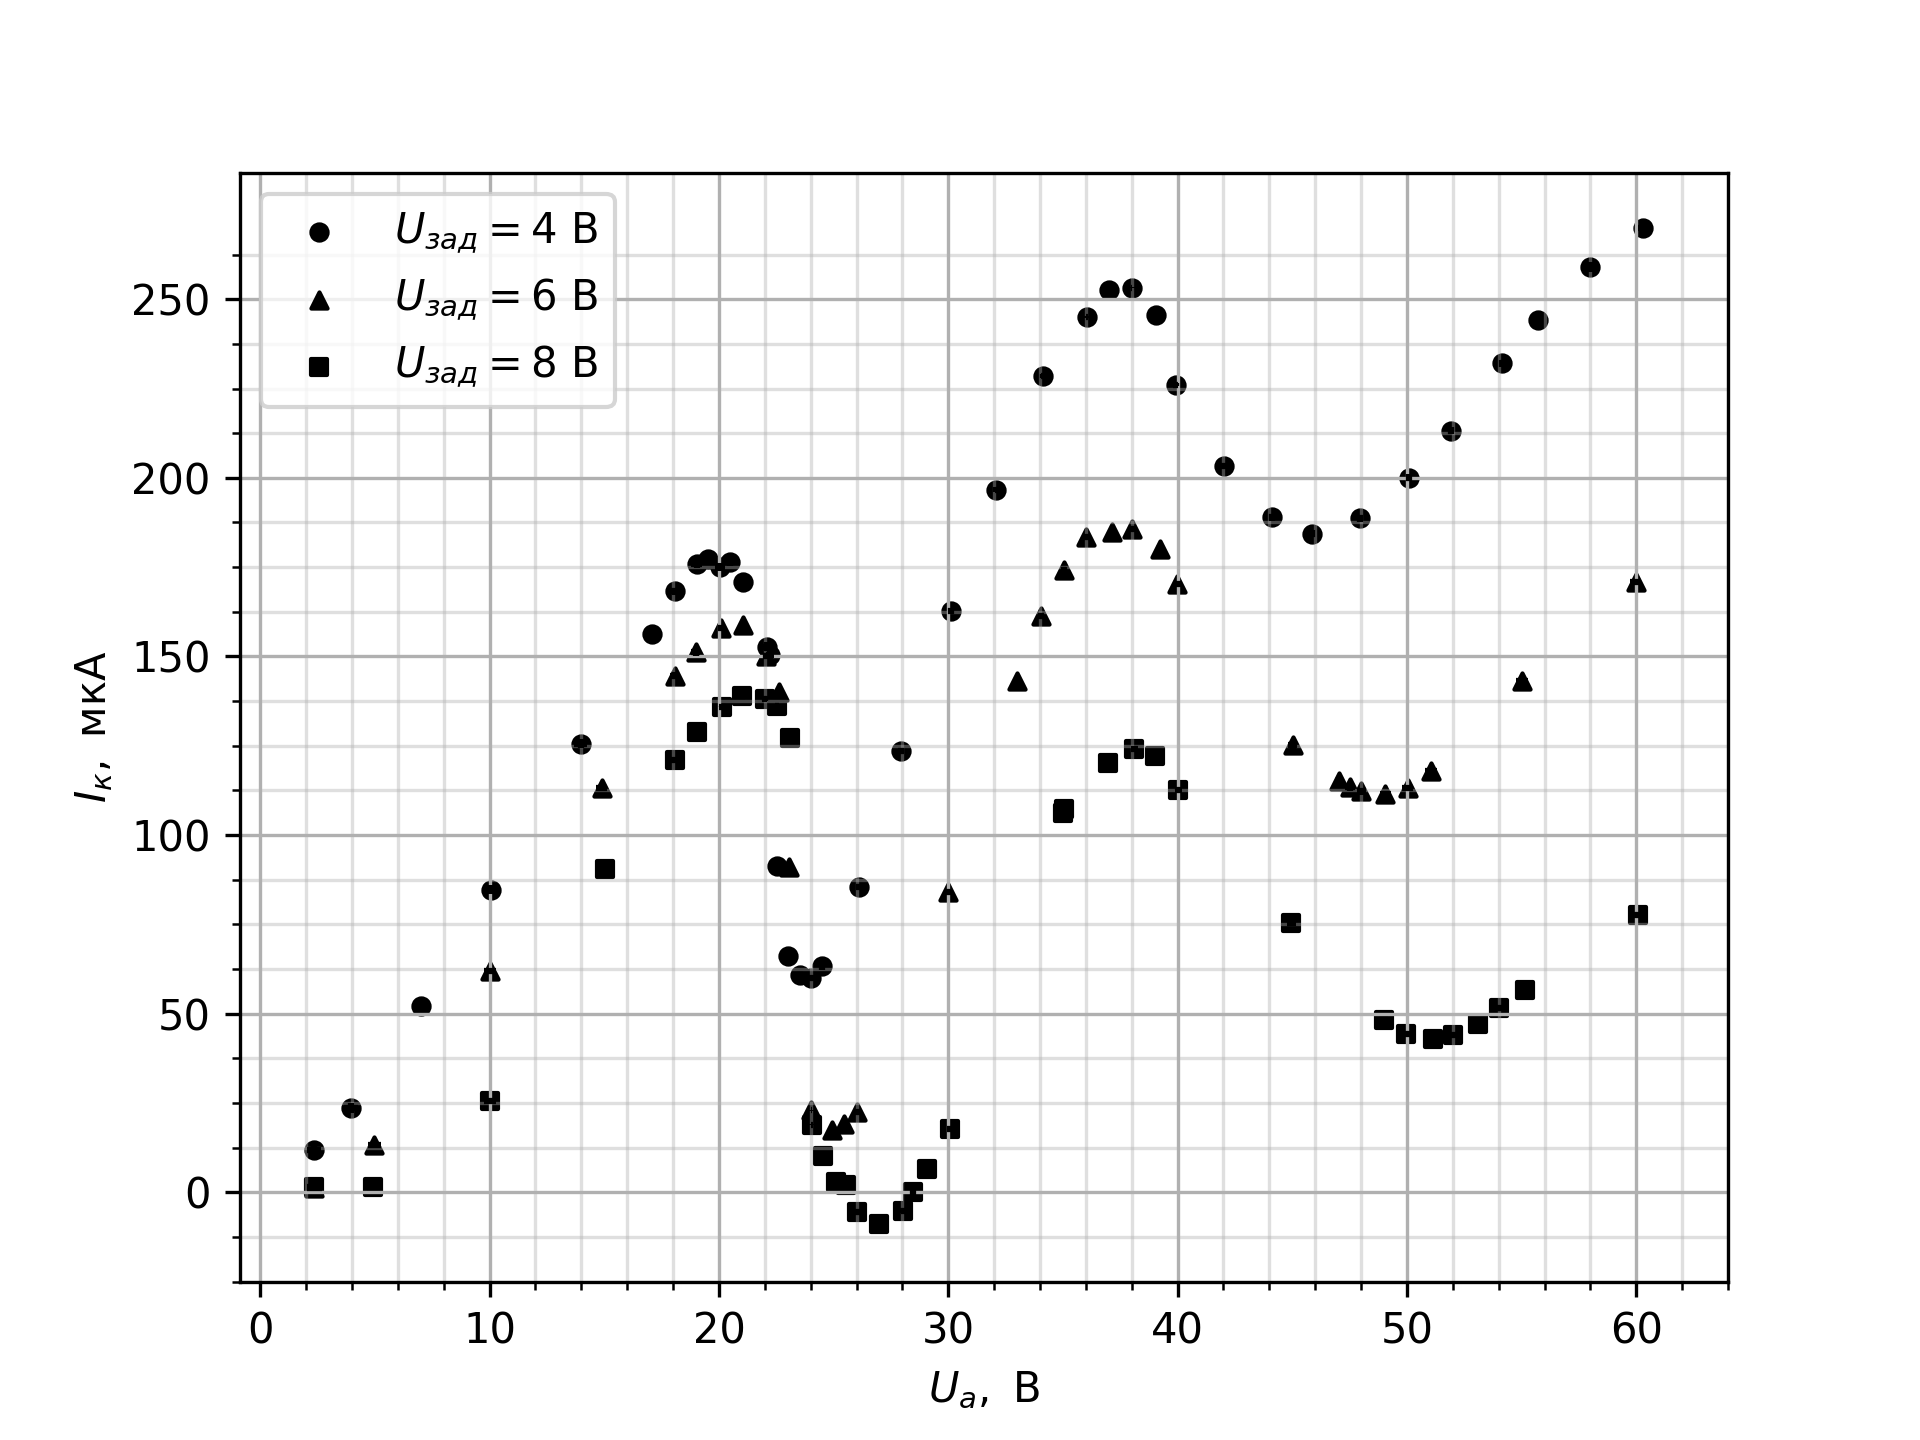
\includegraphics[scale=1]{../images/521-4}
\caption{Зависимость коллекторного тока от анодного напряжения для различных значений задерживающего напряжения}
\end{figure}

\end{enumerate}

\section{Обработка результатов}

Построим графики зависимости $I_к=f(U_а)$ при различных значениях запирающего напряжения. По графикам определим энергию возбуждения первого уровня атома гелия. Для этого аппроксимируем экстремумы зависимости параболами с уравнением

\[I_к=k(U_a-U_0)^2+I_0\text{.}\]

Тогда координата пика вдоль оси $U_a$ будет определяться единственным параметром $U_0$. Из аппроксимации получим следующие значения $\Delta U=U_2-U_1$:

\[\Delta U_1=(17.6\pm0.2)\ В\quad \Delta U_2=(17.0\pm0.2)\ В\quad \Delta U_3=(16.8\pm0.2)\ В\]

Так как положение пиков не зависит от запирающего напряжения, найдем итоговую величину анодного напряжения усреднив полученные значения.

\[\Delta U=\frac{\Delta U_1+\Delta U_2+\Delta U_3}{3}=(17.1\pm0.2)\ В\]

Тогда энергия возбуждения первого уровня атома гелия составляет

\[E=e\Delta U=(17.1\pm0.2)\ эВ\]

\begin{figure}[H]
\centering
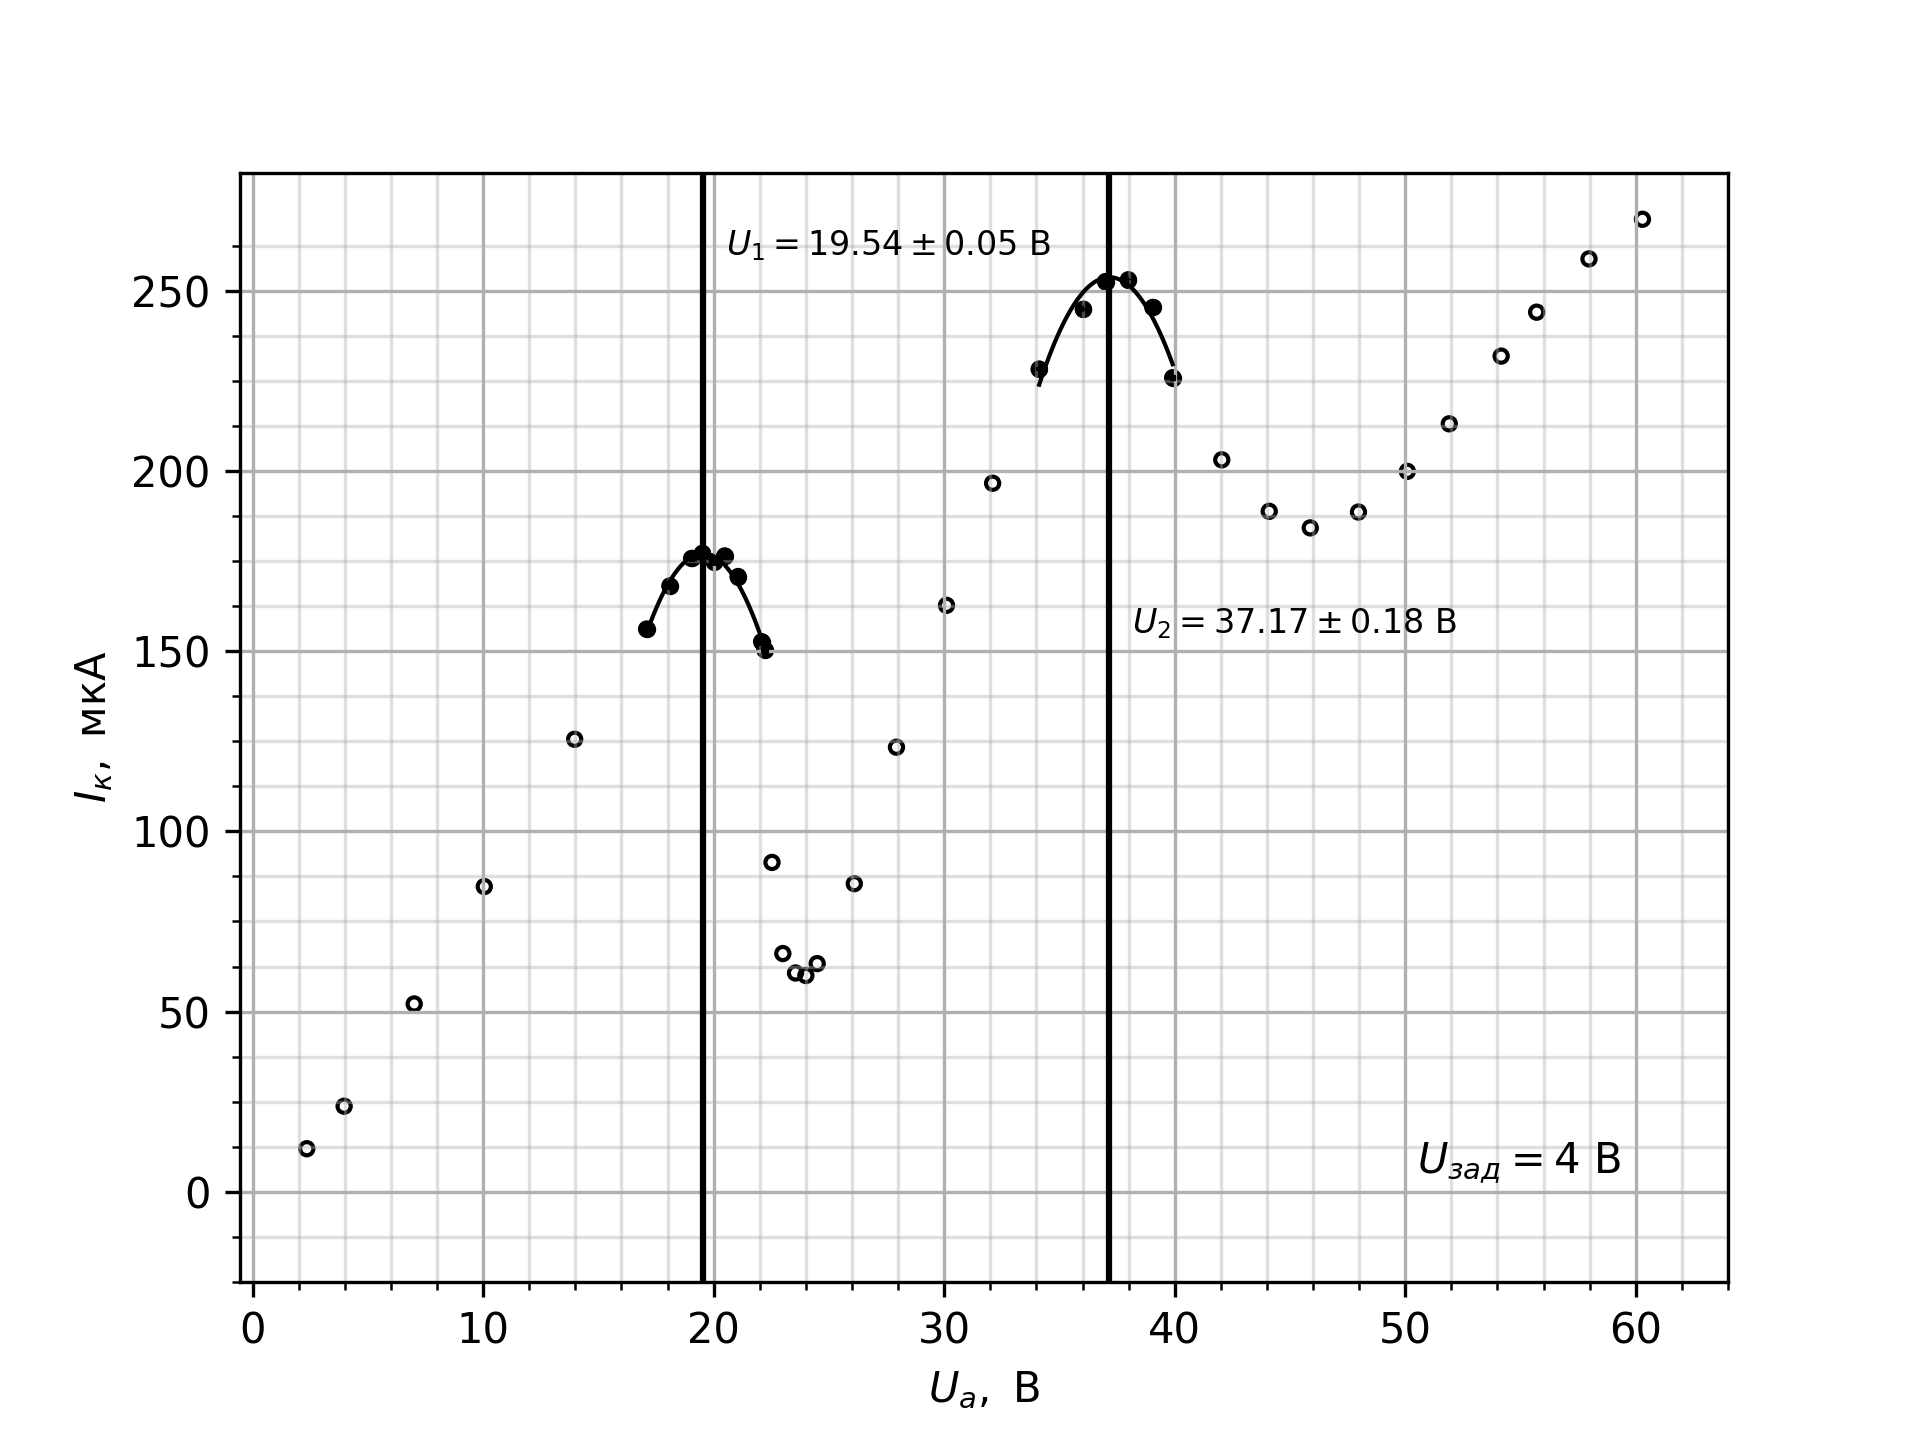
\includegraphics[scale=0.9]{../images/521-5}
\caption{Определение положения экстремумов. $U_{зад}=4\ \text{В}$}
\end{figure}

\begin{figure}[H]
\centering
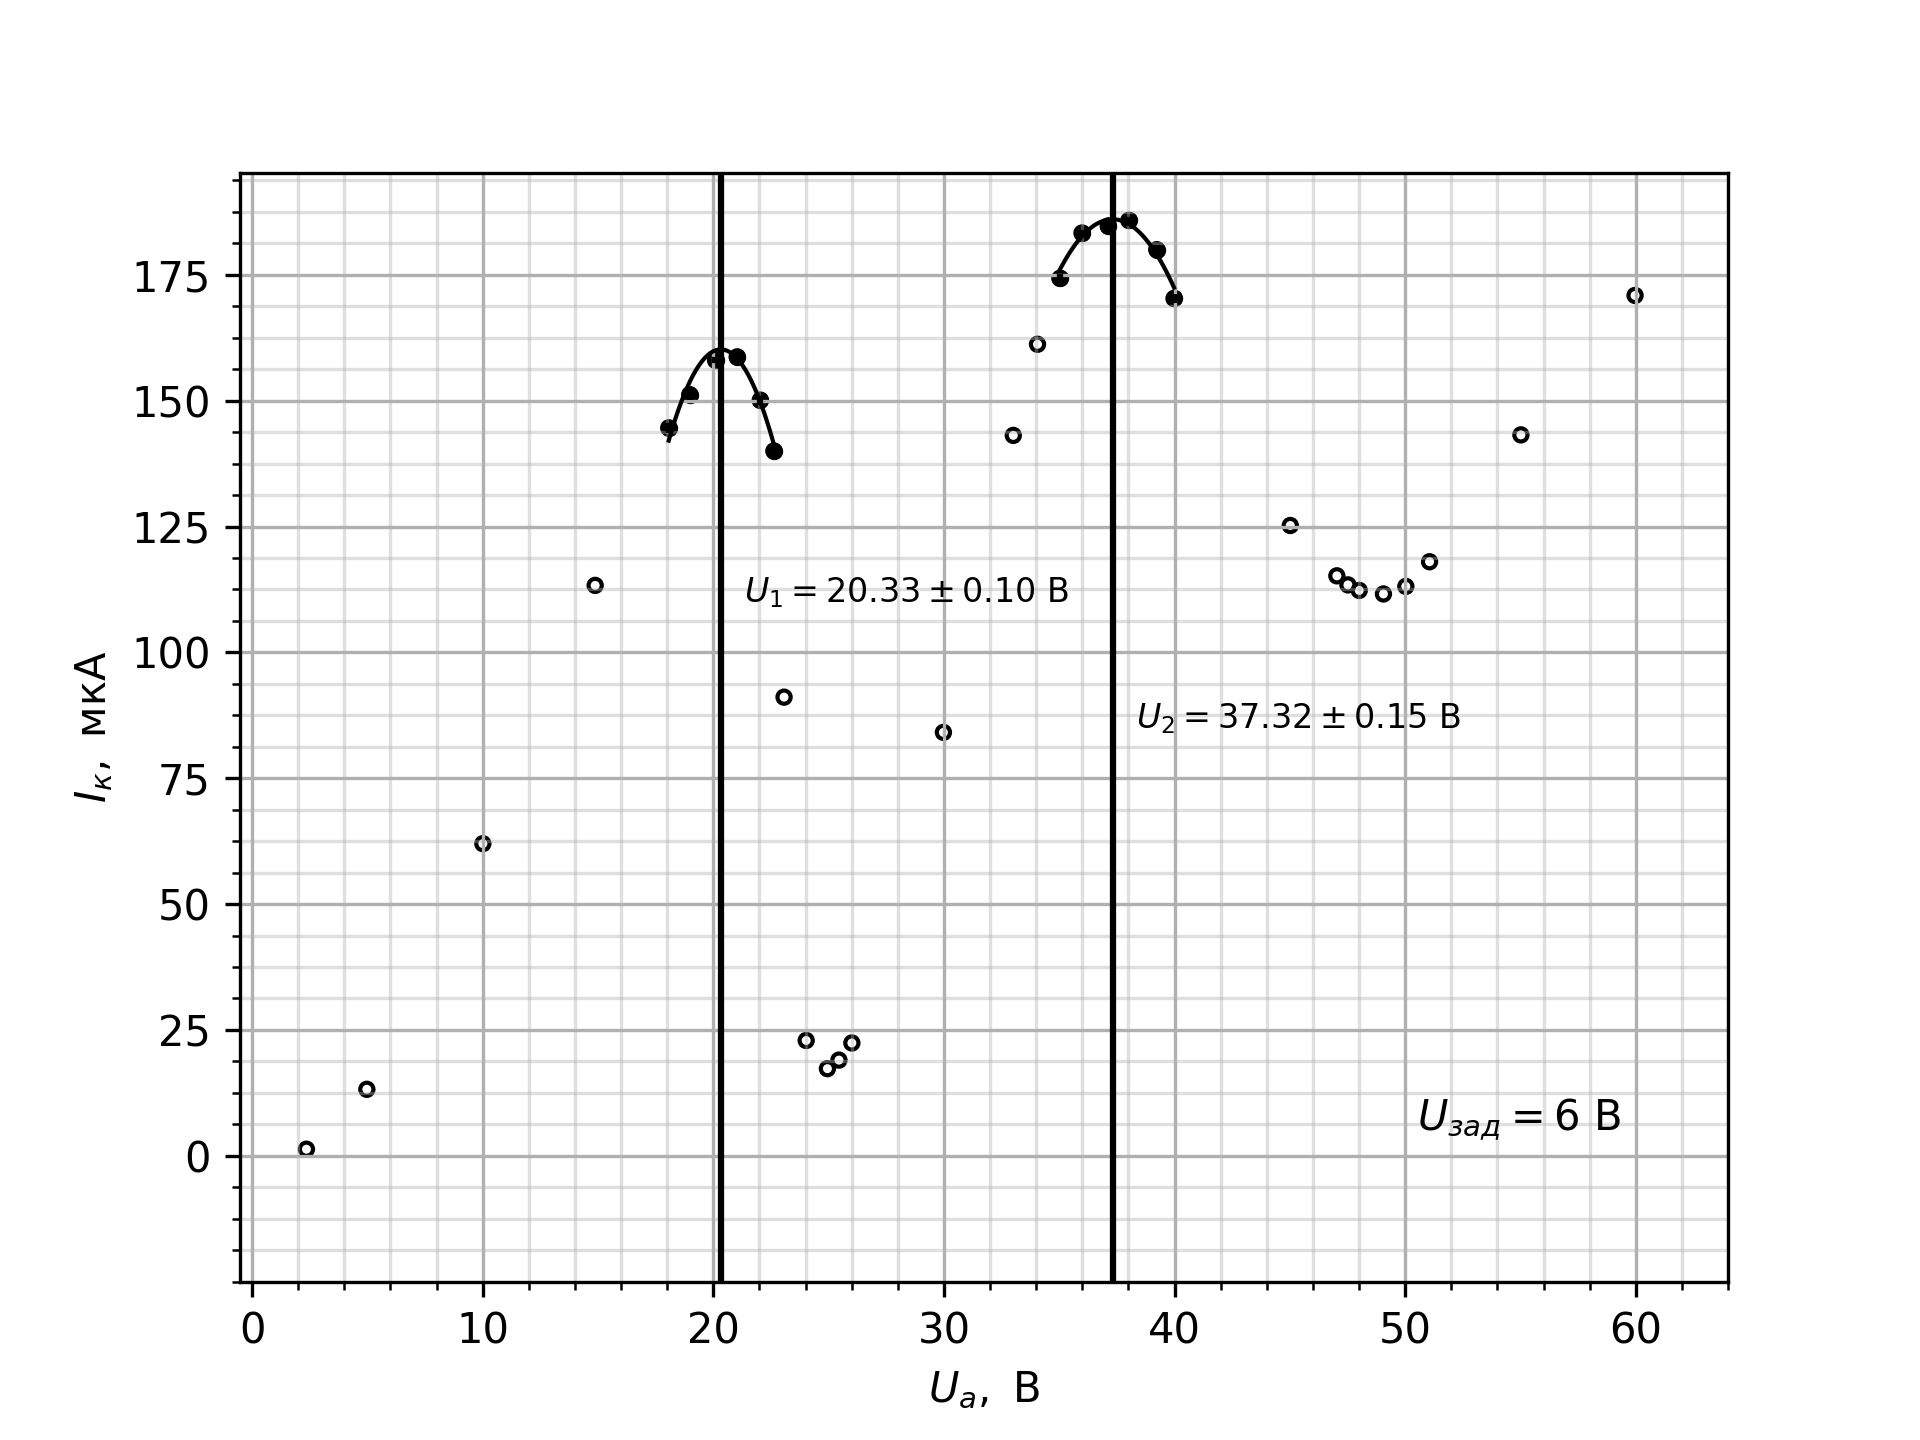
\includegraphics[scale=0.9]{../images/521-6}
\caption{Определение положения экстремумов. $U_{зад}=6\ \text{В}$}
\end{figure}

\begin{figure}[H]
\centering
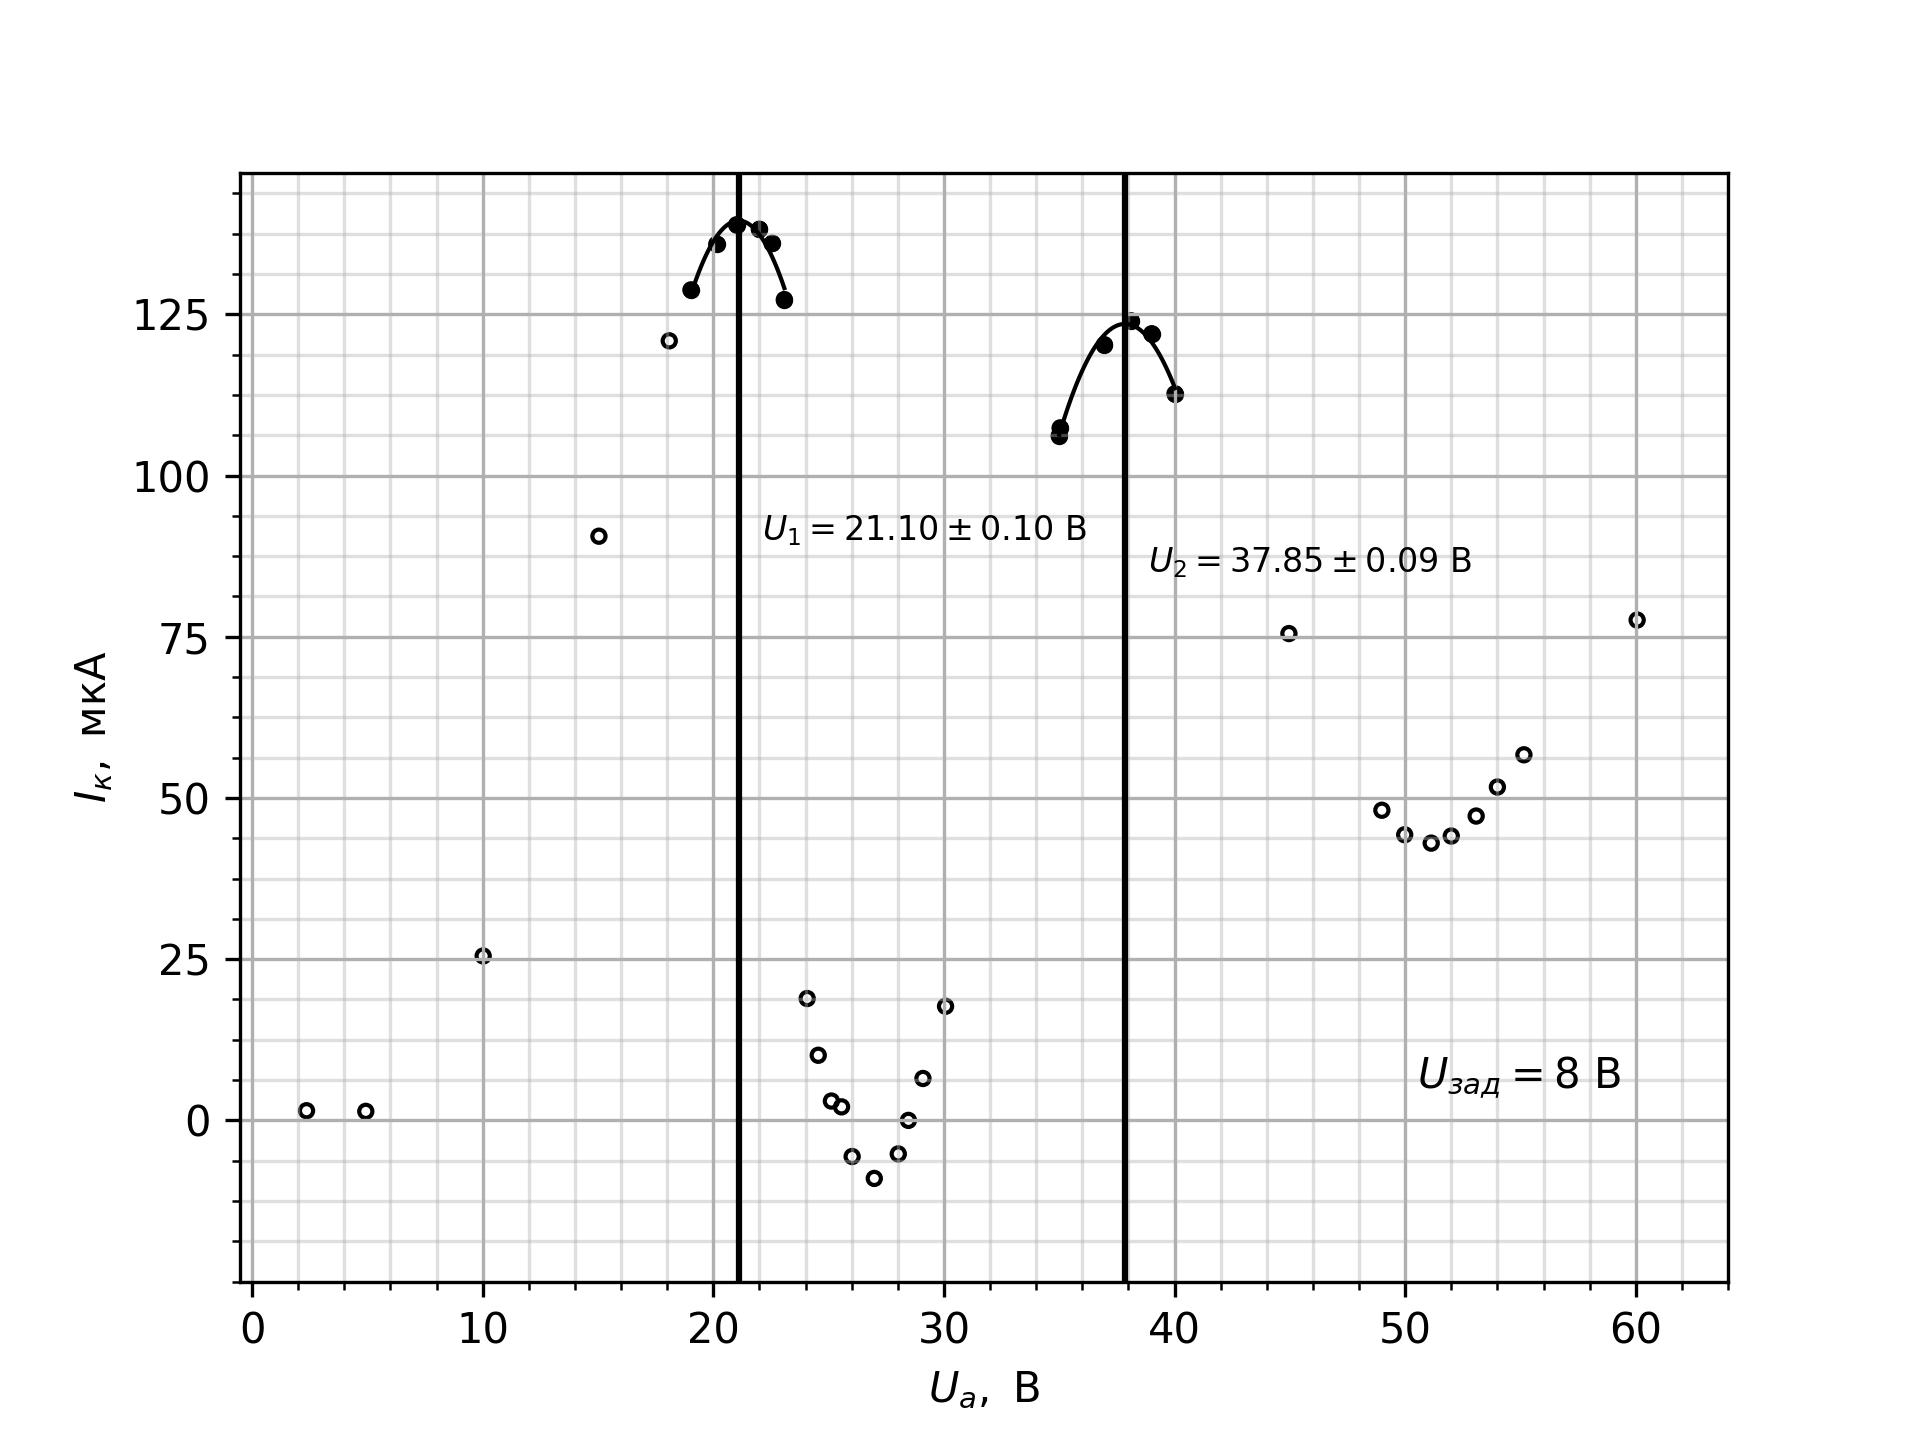
\includegraphics[scale=0.9]{../images/521-7}
\caption{Определение положения экстремумов. $U_{зад}=8\ \text{В}$}
\end{figure}

\section{Выводы}

Табличное значение энергии возбуждения атома гелия составляет $E=20.55\ эВ$, что сравнимо с полученным в ходе результата значения. 

\end{document}